\documentclass[aspectratio=169]{beamer}

% --- Pacotes de Idioma e Codificação ---
\usepackage[utf8]{inputenc}
\usepackage[portuguese]{babel}
\usepackage[T1]{fontenc}
\usepackage{graphicx}
\usepackage{url}
\usepackage{amsmath}
\usepackage{booktabs}
\usepackage{subcaption}
\usepackage{listings}
\usepackage{xcolor}

% --- Tema e Cores Customizadas (UFABC) ---
\usetheme{Madrid}
\usecolortheme{default}

\definecolor{ufabcgreen}{RGB}{0, 79, 0}
\definecolor{ufabcgold}{RGB}{212, 175, 55}
\definecolor{darkgray}{RGB}{50, 50, 50}

\setbeamercolor{palette primary}{bg=ufabcgreen,fg=white}
\setbeamercolor{palette secondary}{bg=ufabcgreen!80!black,fg=white}
\setbeamercolor{palette tertiary}{bg=ufabcgreen!60!black,fg=white}
\setbeamercolor{palette quaternary}{bg=ufabcgreen!40!black,fg=white}
\setbeamercolor{structure}{fg=ufabcgreen}
\setbeamercolor{section in toc}{fg=ufabcgreen}
\setbeamercolor{block title}{bg=ufabcgreen, fg=white}
\setbeamercolor{block body}{bg=ufabcgreen!10!white, fg=darkgray}

% Remover botões de navegação no rodapé
\setbeamertemplate{navigation symbols}{}

% Logo no cabeçalho ou rodapé (opcional)
\titlegraphic{
\includegraphics[width=1.5cm]{Ufabc_logo.png}}

% --- Informações do Trabalho ---
\title[Defesa de PGC - Rust/WASM na Névoa]{Filtro de Dados e Compressão para Computação em Névoa em IoT na Agricultura Inteligente utilizando Rust e WebAssembly}
\author[Victor Cobo Figueiro]{Victor Cobo Figueiro}
\institute[UFABC]{
  Curso de Bacharelado em Ciência da Computação\\
  Universidade Federal do ABC - UFABC
}
\date[Julho de 2026]{Julho de 2026\\ \vspace{0.2cm} \small Orientador: Prof. Dr. Carlos Alberto Kamienski}

% --- Início do Documento ---
\begin{document}

% Slide de Capa
\begin{frame}
  \titlepage
\end{frame}

% Sumário da Apresentação
\begin{frame}{Sumário}
  \tableofcontents
\end{frame}

% ==========================================================
\section{Introdução e Objetivos}
% ==========================================================

\begin{frame}{Introdução e Motivação}
  \begin{itemize}
    \item \textbf{Agricultura Inteligente (Smart Agriculture)}:
      \begin{itemize}
        \item Sensoriamento contínuo de variáveis ambientais (temperatura, umidade, solo).
        \item Auxilia na otimização de recursos (irrigação, defensivos) e prevenção de pragas.
      \end{itemize}
    \vspace{0.3cm}
    \item \textbf{Gargalo de Rede em Ambientes Remotos}:
      \begin{itemize}
        \item Links de comunicação de longo alcance e baixo consumo (\textit{LoRaWAN, satélite}).
        \item Banda passante extremamente limitada e alto custo energético por byte transmitido.
        \item Envio direto de dados brutos à nuvem causa congestionamento e morte prematura das baterias dos sensores.
      \end{itemize}
  \end{itemize}
\end{frame}

\begin{frame}{O Problema da Telemetria IoT}
  \begin{block}{O Paradoxo do Sensoriamento Físico}
    Sensores de temperatura e umidade emitem leituras decimais redundantes de alta frequência. Enviar continuamente dados flutuantes decimais (ex: \texttt{24.53, 60.12}) satura canais de rádio de baixa taxa sem agregar valor agronômico direto instantâneo.
  \end{block}
  \vspace{0.3cm}
  \textbf{Desafios:}
  \begin{enumerate}
    \item Reduzir o volume de dados na ponta da rede (Thing e Névoa).
    \item Manter a relevância agronômica das informações transmitidas.
    \item Viabilizar uma arquitetura de orquestração leve no contínuo IoT-Nuvem.
  \end{enumerate}
\end{frame}

\begin{frame}{Objetivos do Trabalho}
  \begin{itemize}
    \item \textbf{Geral}: Propor, implementar e avaliar um ecossistema distribuído de computação em névoa baseado em \textbf{Rust} e \textbf{WebAssembly (WASM/WASI)} para filtragem e compressão de dados na borda.
    \vspace{0.2cm}
    \item \textbf{Específicos}:
      \begin{enumerate}
        \item Adaptar o classificador $k$-Vizinhos Mais Próximos ($k$NN, com $k=3$) para converter medidas físicas de temperatura e umidade em status de saúde do tomateiro de caractere único.
        \item Avaliar a compressão temporal via codificação RLE (*Run Length Encoding*).
        \item Projetar um simulador estocástico off-line (KDE + Box-Muller) para validar estatisticamente a robustez do ecossistema.
        \item Medir a eficácia e o consumo de rede comparativo das diferentes configurações de buffer.
      \end{enumerate}
  \end{itemize}
\end{frame}

% ==========================================================
\section{Referencial Teórico}
% ==========================================================

\begin{frame}{Computação em Névoa e o IoTinuum}
  \begin{itemize}
    \item \textbf{Computação em Névoa (Fog Computing)}:
      \begin{itemize}
        \item Camada intermediária que descentraliza a computação da Nuvem para locais próximos aos sensores.
        \item Mitiga latência, economiza banda passante de uplink e viabiliza resposta ágil no campo.
      \end{itemize}
    \vspace{0.3cm}
    \item \textbf{O Cloud Continuum (IoTinuum)}:
      \begin{itemize}
        \item Orquestração unificada de cargas lógicas que trafegam entre as camadas de \textit{Things}, \textit{Edge/Fog} e \textit{Cloud}.
        \item \textbf{Problema de Orquestradores Clássicos (Docker/K8s/KubeEdge)}: Pegada de memória e CPU muito pesada para nós de borda fracos (gateways agrícolas de baixo custo).
      \end{itemize}
  \end{itemize}
\end{frame}

\begin{frame}{Rust e WebAssembly (WASM/WASI) na Névoa}
  \begin{itemize}
    \item \textbf{WebAssembly (WASM)}:
      \begin{itemize}
        \item Formato de instrução binária de baixo nível executado em máquina virtual baseada em pilha com isolamento estrito (\textit{sandboxing}).
        \item \textit{WebAssembly System Interface} (WASI) padroniza o acesso seguro a recursos do hospedeiro.
      \end{itemize}
    \vspace{0.3cm}
    \item \textbf{Benefícios Frente a Soluções Tradicionais (Containers/JVM)}:
      \begin{itemize}
        \item \textbf{Velocidade Quase Nativa}: Sobrecarga do bytecode WASM com JIT/AOT é de apenas 1,1x a 1.5x do código nativo compilado.
        \item \textbf{Footprint Mínimo}: Tamanho de imagem em KBs (vs Megabytes de Docker) e instanciamento em microssegundos (sem overhead de cold start).
        \item \textbf{Segurança Baseada em Capabilidades}: Bloqueio de rede e E/S por padrão, liberados explicitamente via flags do runtime (ex: WasmEdge).
      \end{itemize}
  \end{itemize}
\end{frame}

\begin{frame}{Trabalho de Base e Diferenciais}
  \begin{itemize}
    \item \textbf{Fundamentação Teórica (Ribeiro Junior et al., 2020)}:
      \begin{itemize}
        \item Concebeu a modelagem matemática e a lógica do filtro $k$NN com RLE aplicado a dados climáticos de tomateiros.
      \end{itemize}
    \vspace{0.3cm}
    \item \textbf{Avanços e Diferenciais Introduzidos neste PGC}:
      \begin{enumerate}
        \item \textbf{Implementação Prática Real}: Migração do escopo analítico puro para um ecossistema distribuído completo em Rust e WASM rodando no runtime WasmEdge.
        \item \textbf{Validação Estatística Offline}: Desenvolvimento nativo de um gerador estocástico bivariado via estimador KDE e transformada de Box-Muller em Rust/WASM.
        \item \textbf{Emulação Multiambiente}: Configuração de proxies e servidores para avaliação do impacto físico em rede ao deslocar o processador entre as camadas (Thing, Fog e Cloud).
      \end{enumerate}
  \end{itemize}
\end{frame}

% ==========================================================
\section{Arquitetura e Implementação}
% ==========================================================

\begin{frame}{Arquitetura do Ecossistema Distribuído}
  \begin{figure}[H]
    \centering
    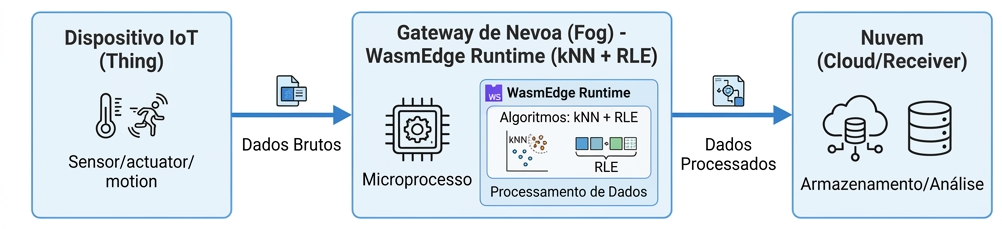
\includegraphics[width=12cm]{esquema_logico.png}
    \caption{Arquitetura lógica em três fases: Thing, Edge/Fog e Cloud.}
    \label{fig:esquema_logico}
  \end{figure}
\end{frame}

\begin{frame}{Algoritmos de Processamento na Névoa}
  \begin{itemize}
    \item \textbf{Filtragem via k-NN (k=3)}:
      \begin{itemize}
        \item Normalização Min-Max em tempo real:
          \[x'_{norm} = \frac{x - x_{min}}{x_{max} - x_{min}}\]
        \item Distância Euclidiana bidimensional para classificar status agronômico do tomateiro em 11 classes (Tabela agronômica baseada no ciclo da cultura).
      \end{itemize}
    \vspace{0.2cm}
    \item \textbf{Compressão Run Length Encoding (RLE)}:
      \begin{itemize}
        \item Transforma strings sequenciais repetitivas de classes de caractere único em contadores e identificadores.
        \item Exemplo: O sinal contínuo \texttt{OOOOWWWAA} de 9 bytes é reduzido para \texttt{4O3W2A} (6 bytes), economizando banda passante em transmissões por buffer temporal.
      \end{itemize}
  \end{itemize}
\end{frame}

\begin{frame}{Detalhes de Implementação e Sandbox}
  \begin{itemize}
    \item \textbf{Linguagem Rust e Bibliotecas}:
      \begin{itemize}
        \item \textbf{Hyper / Reqwest}: Para comunicação HTTP cliente/servidor assíncrona baseada em sockets WASI compatíveis com o WasmEdge.
        \item \textbf{CSV / Serde}: Leitura de alta performance de dados brutos e serialização JSON estruturada ultraleve.
      \end{itemize}
    \vspace{0.3cm}
    \item \textbf{Sandbox WasmEdge e Segurança}:
      \begin{itemize}
        \item Mapeamento explícito de diretórios pela flag \texttt{--dir .} para dar permissão controlada de E/S de arquivos (leitura de datasets e persistência de relatórios).
        \item Ambiente isolado que impede ataques de estouro de buffer ou acesso irrestrito ao sistema operacional hospedeiro.
      \end{itemize}
  \end{itemize}
\end{frame}

% ==========================================================
\section{Metodologia Experimental}
% ==========================================================

\begin{frame}{Metodologia de Teste e Dataset}
  \begin{itemize}
    \item \textbf{Base de Dados Física Real (\texttt{entrada.csv})}:
      \begin{itemize}
        \item $44.023$ registros climáticos bivariados coletados com taxa de amostragem de 5 segundos.
      \end{itemize}
    \vspace{0.3cm}
    \item \textbf{Buffers de Transmissão Avaliados}:
      \begin{itemize}
        \item Cinco janelas de lotes temporais simuladas: \textbf{6} registros (30s), \textbf{60} (5min), \textbf{720} (1h), \textbf{4.320} (6h) e \textbf{20.000} (27,7h).
      \end{itemize}
    \vspace{0.3cm}
    \item \textbf{Cenário de Execução}:
      \begin{itemize}
        \item Emulação executada em distribuição Ubuntu Linux via subsistema WSL em máquina pessoal equipada com Windows 11.
      \end{itemize}
  \end{itemize}
\end{frame}

\begin{frame}{Simulador Estocástico (KDE + Box-Muller)}
  \begin{block}{Objetivo do Gerador em Rust}
    Validar se o ecossistema e o classificador agronômico se comportam de forma consistente sob dados estocásticos modelados a partir do ambiente climático original.
  \end{block}
  \vspace{0.1cm}
  \begin{itemize}
    \item \textbf{Ajuste Estatístico (Offline - KDE)}: Ajuste da curva bivariada de densidade por estimador KDE gaussiano ($h=0.5$) em Python.
      \begin{itemize}
        \item \small \textit{KDE (O "Cérebro"): Mapeia o relevo de probabilidade e a correlação conjunta real do clima.}
      \end{itemize}
    \item \textbf{Amostragem em Rust/WASM (Box-Muller)}: Geração de $40.000$ pontos sintéticos utilizando a transformada Box-Muller:
      \[Z_0 = \sqrt{-2\ln U_1}\cos(2\pi U_2)\]
      \begin{itemize}
        \item \small \textit{Box-Muller (O "Motor"): Transforma números planos (uniformes) em ruído normal (sino) ao redor do relevo.}
        \item \small $U_1, U_2$: Variáveis uniformes independentes em $(0, 1]$, geradas pelo WasmEdge.
        \item \small $Z_0$: Ruído com distribuição normal padrão $N(0, 1)$ adicionado ao ponto base.
      \end{itemize}
  \end{itemize}
\end{frame}

% ==========================================================
\section{Resultados e Discussões}
% ==========================================================

\begin{frame}{Validação Estatística do Gerador em Rust}
  \begin{itemize}
    \item \textbf{Teste de Kolmogorov-Smirnov (Duas Amostras)}:
      \begin{itemize}
        \item Temperatura: estatística de $0,0081$ e \textbf{p-valor de $0,1385$}.
        \item Umidade: estatística de $0,0041$ e \textbf{p-valor de $0,8974$}.
        \item \small \textit{\textbf{p-valor (KS-Test)}: Mede a probabilidade de as amostras virem da mesma distribuição. Se $p > 0,05$ (limite crítico), provamos que os dados reais e sintéticos são estatisticamente indistinguíveis.}
      \end{itemize}
    \vspace{0.1cm}
    \item \textbf{Correlação Linear (Pearson $r$)}:
      \begin{itemize}
        \item Correlação Real: $-0,6429$.
        \item Correlação Sintética (Rust): $-0,6396$ (Desvio absoluto: $0,0033$).
        \item \small \textit{\textbf{Pearson r}}: Mede o quanto as variáveis caminham juntas. O valor negativo ($\approx -0,64$) reflete a física real do clima (temperatura sobe $\to$ umidade desce), perfeitamente preservada pelo gerador.
      \end{itemize}
  \end{itemize}
\end{frame}

\begin{frame}{Análise Visual: Curvas de Densidade Conjunta}
  \begin{figure}[H]
    \centering
    \begin{subfigure}[b]{0.45\textwidth}
      \centering
      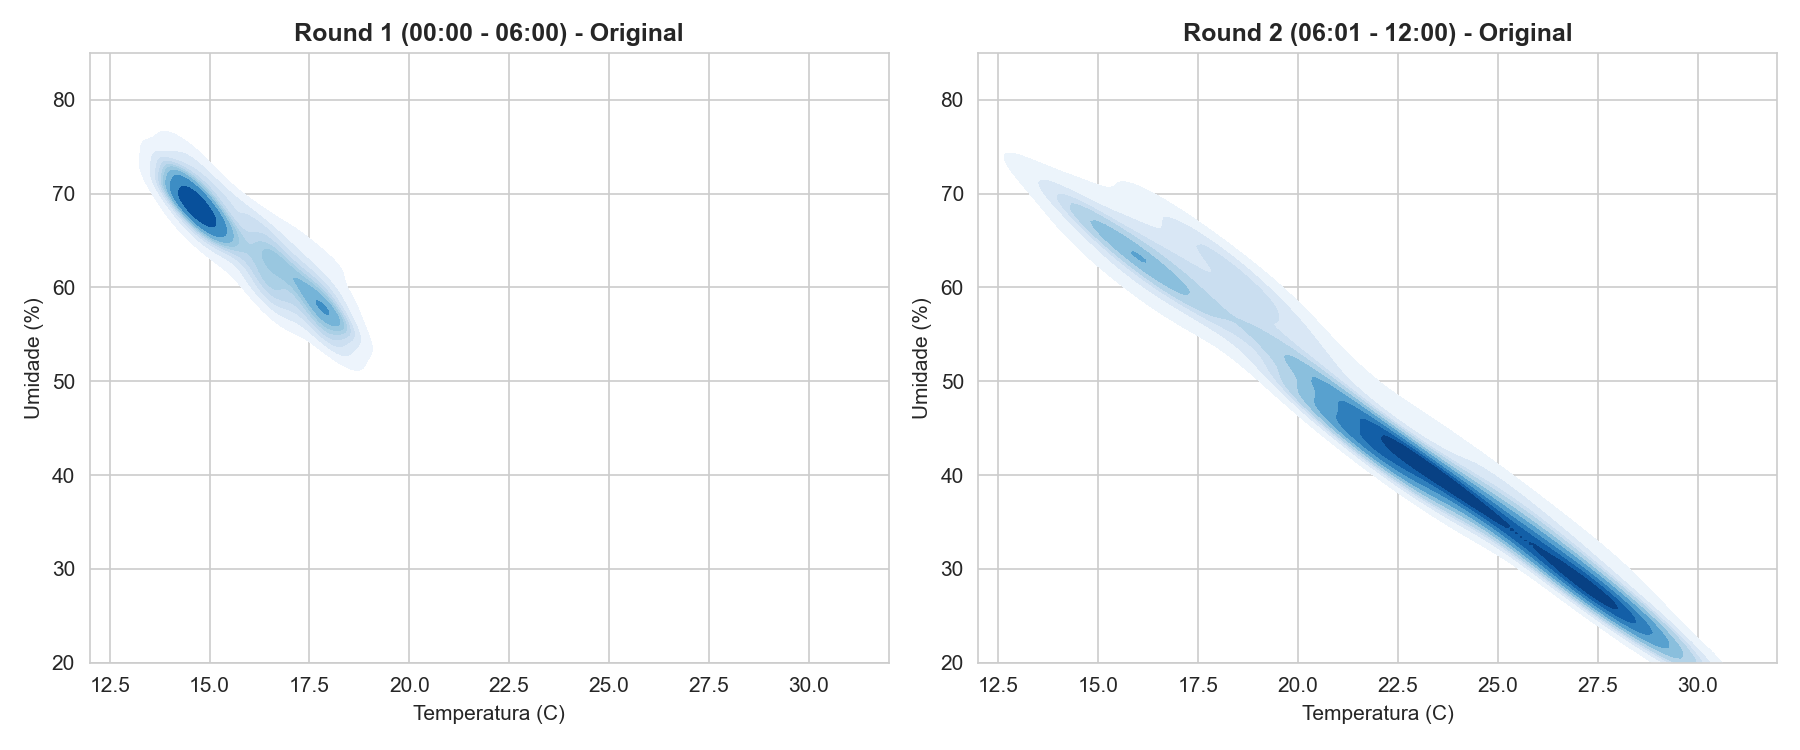
\includegraphics[width=4.0cm]{analise-experimentos/densidade_artigo_original.png}
      \caption{Base Real (\texttt{entrada.csv})}
    \end{subfigure}
    \hfill
    \begin{subfigure}[b]{0.45\textwidth}
      \centering
      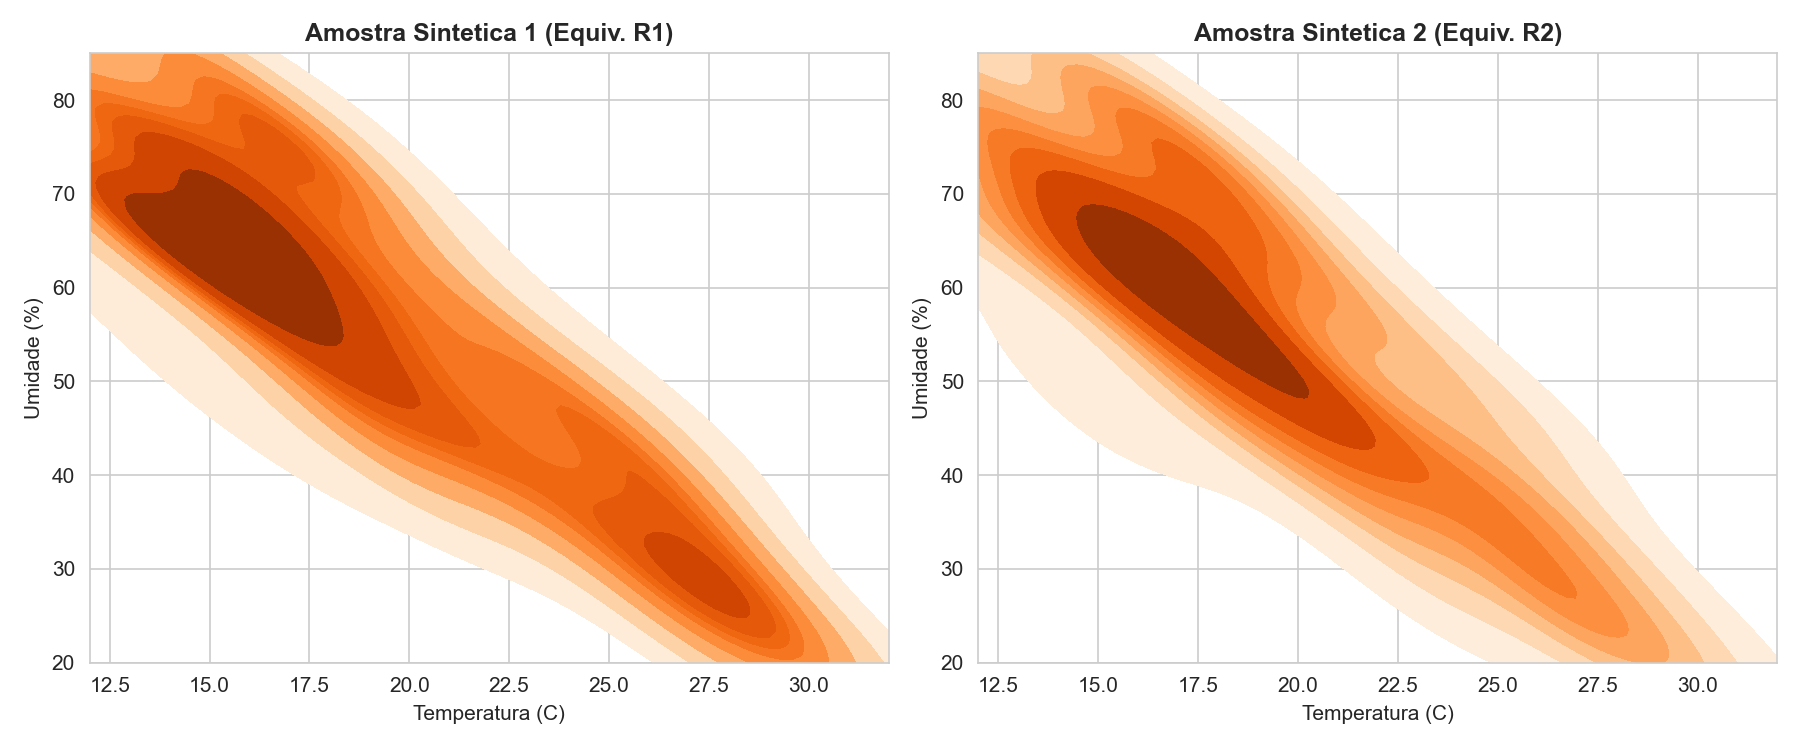
\includegraphics[width=4.0cm]{analise-experimentos/densidade_artigo_sintetico.png}
      \caption{Base Sintética (Rust/WASM)}
    \end{subfigure}
    \caption{Comparativo das curvas de contorno de densidade de probabilidade conjunta.}
    \label{fig:curvas_densidade}
  \end{figure}
  \vspace{-0.4cm}
  \begin{itemize}
    \item \small As metades sintéticas (Amostras 1 e 2) são idênticas entre si e cobrem a amplitude diagonal global. Isso ocorre porque o gerador KDE é um modelo probabilístico estático e \textit{i.i.d.} (não modela a ordenação cronológica temporal da série física original).
  \end{itemize}
\end{frame}

\begin{frame}{Análise Visual: Correlogramas e Dispersão Cruzada}
  \begin{figure}[H]
    \centering
    \begin{subfigure}[b]{0.48\textwidth}
      \centering
      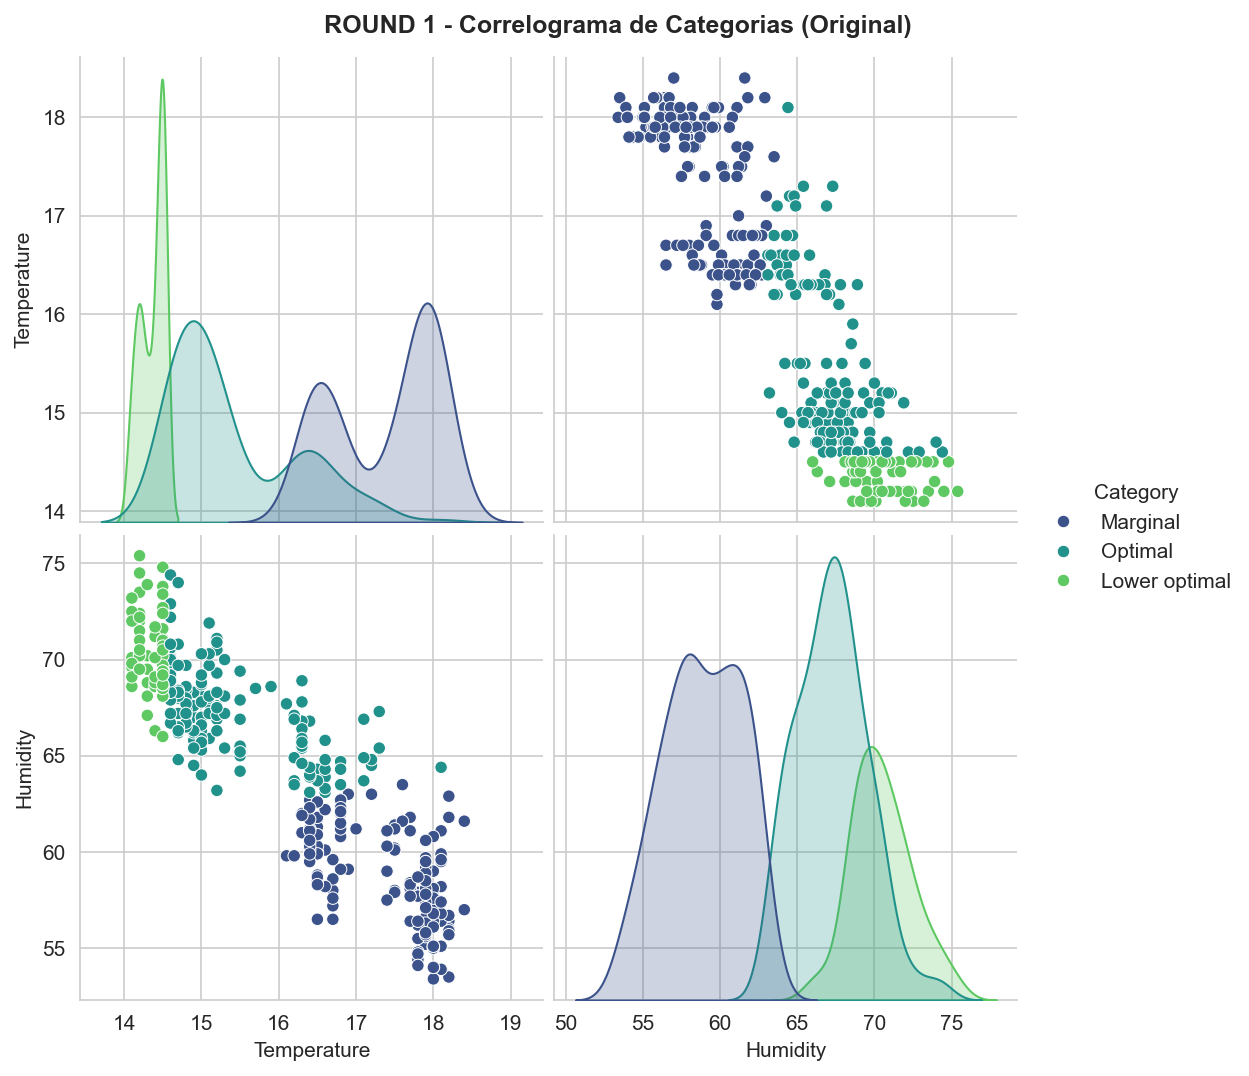
\includegraphics[width=4.2cm]{analise-experimentos/correlograma_r1_original.png}
      \caption{Round 1 - Original}
    \end{subfigure}
    \hfill
    \begin{subfigure}[b]{0.48\textwidth}
      \centering
      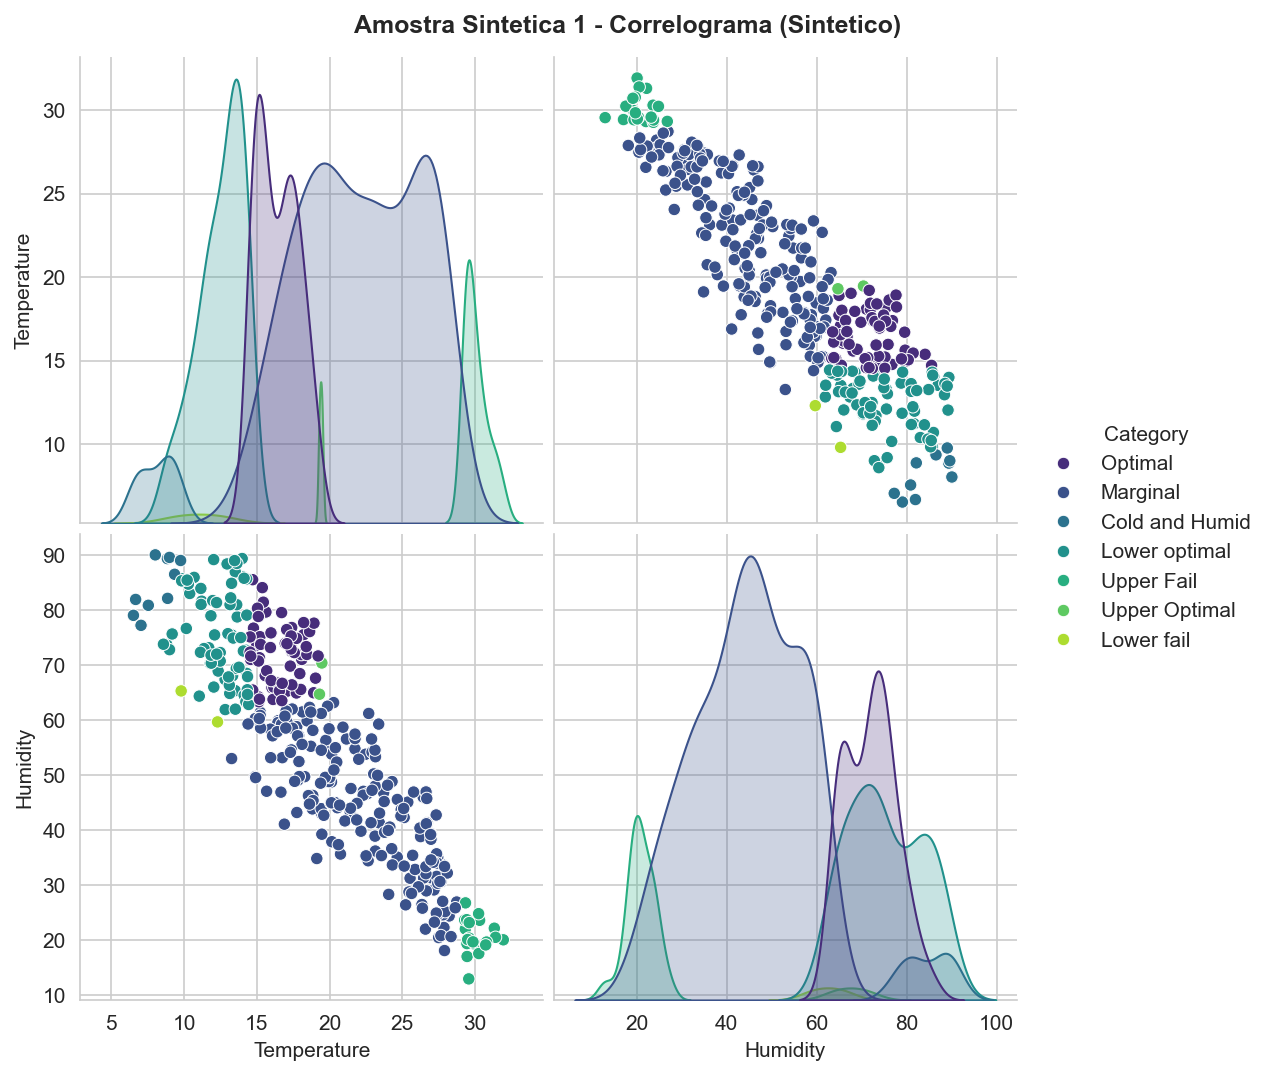
\includegraphics[width=4.2cm]{analise-experimentos/correlograma_r1_sintetico.png}
      \caption{Round 1 - Sintético}
    \end{subfigure}
    \caption{Correlogramas de Temperatura vs Umidade classificados por kNN (Round 1).}
    \label{fig:correlograma_r1}
  \end{figure}
  \vspace{-0.4cm}
  \begin{itemize}
    \item \small Enquanto o Round 1 real concentra-se em 14 a 19$^\circ$C (ativando 3 classes kNN), o sintético dispersa-se por todo o espectro global (5 a 30$^\circ$C) e ativa classes adicionais, pois a amostragem aleatória do KDE reflete a densidade global conjunta.
  \end{itemize}
\end{frame}

\begin{frame}{Análise Visual: Densidade Global Completa}
  \begin{figure}[H]
    \centering
    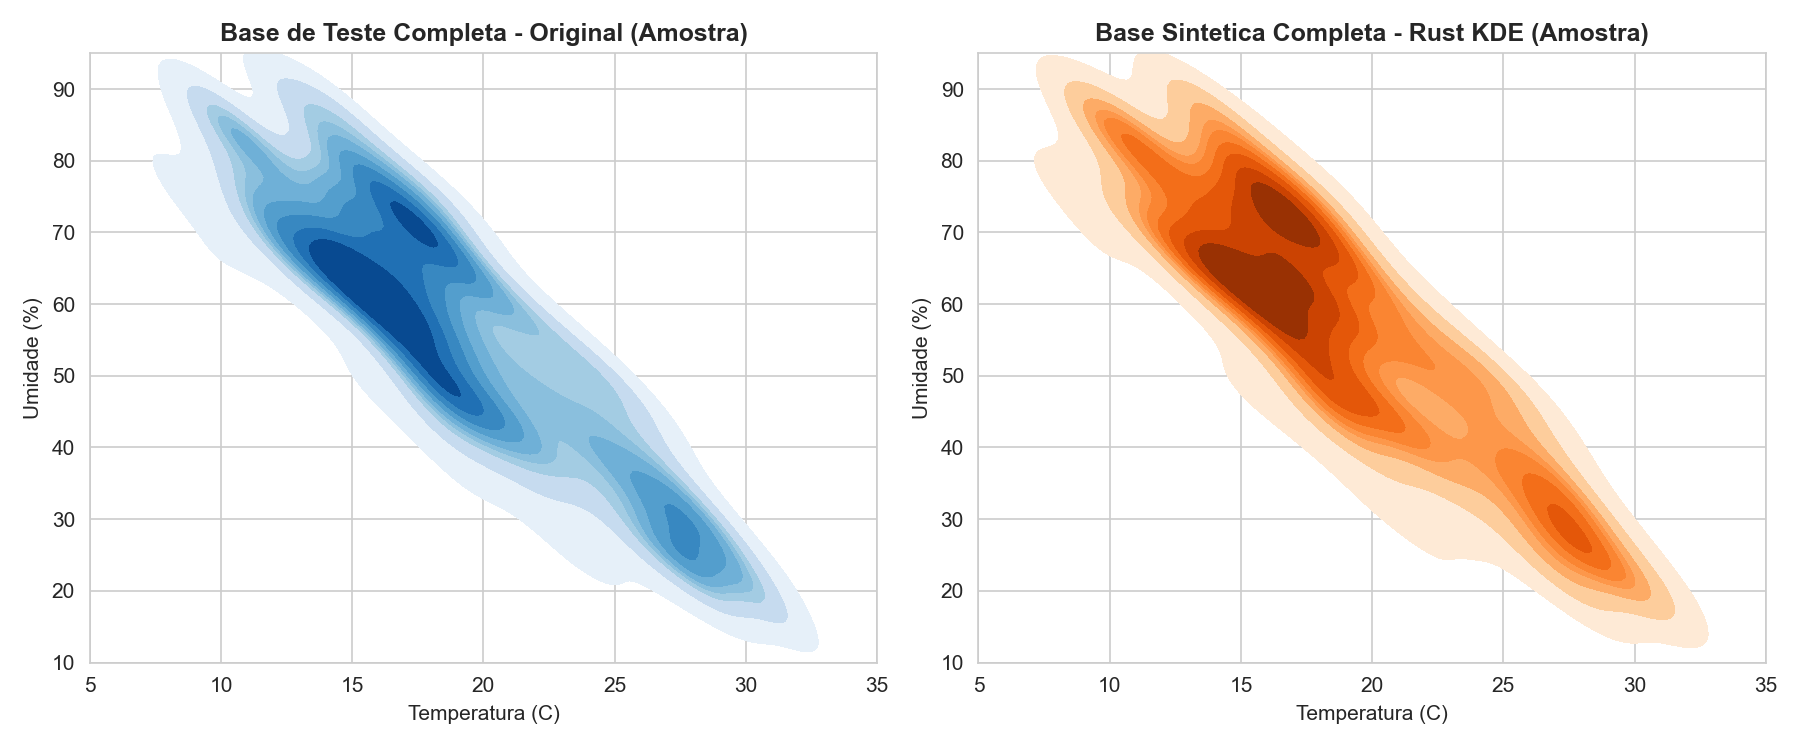
\includegraphics[width=7.0cm]{analise-experimentos/densidade_global_comparacao.png}
    \caption{Comparação de Densidade Bidimensional Completa (Original vs Sintético).}
    \label{fig:densidade_global_slide}
  \end{figure}
  \vspace{-0.4cm}
  \begin{itemize}
    \item \small Sob a perspectiva global, o gerador KDE em Rust recupera a estrutura estocástica latente com altíssima fidelidade, com contornos e centros de adensamento muito próximos à base real.
    \item \small Contudo, a perda de ordenação temporal (modelo \textit{i.i.d.}) introduz ruído de alta frequência na série sintética. Isso reduz as sequências de repetição e explica a menor eficiência do RLE nos dados simulados.
  \end{itemize}
\end{frame}

\begin{frame}{Resultados de Eficiência de Compressão}
  \begin{table}[h]
    \centering
    \caption{Tamanho médio acumulado e redução de dados por tamanho de lote.}
    \label{tab:compressao_lote}
    \resizebox{0.8\textwidth}{!}{%
    \begin{tabular}{ccccc}
      \toprule
      \textbf{Tamanho Lote} & \textbf{Original (B)} & \textbf{kNN Puro (B)} & \textbf{kNN+RLE (B)} & \textbf{Redução kNN+RLE (\%)} \\ \midrule
      6 & 222 & 6 & 11,8 & 94,68\% \\
      60 & 2.222 & 60 & 75,7 & 96,59\% \\
      720 & 26.732 & 720 & 814,6 & 96,95\% \\
      4.320 & 160.392 & 4.320 & 4.908,4 & 96,93\% \\
      20.000 & 742.668 & 20.000 & 22.842,5 & 96,92\% \\ \bottomrule
    \end{tabular}%
    }
  \end{table}
  \vspace{-0.1cm}
  * A redução máxima observada foi do \textbf{kNN Puro (estável em 97,84\%)}, superando o kNN+RLE.
\end{frame}

\begin{frame}{Discussão: Fenômeno de Expansão de Símbolo Único}
  \begin{block}{O que explica a ineficiência do RLE?}
    A codificação RLE opera agrupando sequências de caracteres repetitivos (ex: \texttt{3O} para três status Ótimo consecutivos). Contudo, devido à variabilidade natural e ruídos físicos de alta frequência dos sensores climáticos de campo, os caracteres alternam-se rapidamente no buffer.
  \end{block}
  \vspace{0.2cm}
  * \textbf{Expansão de Símbolo Único}: Se não há repetições sequenciais de categorias e elas alternam a cada passo, o RLE precisa emitir um contador \texttt{1} para cada caractere (ex: a cadeia de 3 bytes \texttt{O W A} torna-se \texttt{1O1W1A}, consumindo 6 bytes).
  * \textbf{Diretriz de Projeto}: Em alfabetos curtos sob ruído de sensores físicos, a compressão de entropia RLE gera sobrecarga de rede, sendo mais eficiente transmitir apenas a saída bruta rotulada de caractere único do kNN.
\end{frame}

% ==========================================================
\section{Conclusões}
% ==========================================================

\begin{frame}{Conclusões}
  \begin{itemize}
    \item \textbf{Viabilidade Tecnológica}:
      \begin{itemize}
        \item Rust e WebAssembly (WASM/WASI) provaram-se altamente eficientes e leves para estruturar a computação descentralizada em nós de névoa agrícolas.
      \end{itemize}
    \vspace{0.2cm}
    \item \textbf{Filtragem e Compressão}:
      \begin{itemize}
        \item O kNN atuou como um excelente pré-filtro semântico, reduzindo os dados climáticos reais em \textbf{97,84\%} de volume de payload bruto de telemetria.
        \item A combinação com RLE mostrou-se contraprodutiva para buffers temporais menores devido ao ruído físico dos sensores.
      \end{itemize}
    \vspace{0.2cm}
    \item \textbf{Validação Estocástica}:
      \begin{itemize}
        \item O gerador bivariado em Rust/WASM replicou com sucesso e alta consistência estatística (p-valor de KS $> 0.05$) as propriedades de variabilidade do clima real.
      \end{itemize}
  \end{itemize}
\end{frame}

\begin{frame}{Trabalhos Futuros}
  \begin{enumerate}
    \item \textbf{Orquestração Dinâmica de Tarefas (Workload Migration)}:
      \begin{itemize}
        \item Implementar mecanismos em WASM para migrar a lógica do processamento (kNN) do Thing para a Névoa de forma autônoma e dinâmica de acordo com a oscilação da banda LoRaWAN.
      \end{itemize}
    \vspace{0.2cm}
    \item \textbf{Validação em Hardware Físico Embarcado}:
      \begin{itemize}
        \item Avaliar a performance do WasmEdge rodando em nós microcontroladores de campo reais baseados em ESP32 ou Raspberry Pi Zero.
      \end{itemize}
    \vspace{0.2cm}
    \item \textbf{Algoritmos de Compressão Adaptativos}:
      \begin{itemize}
        \item Investigar a utilização de outros codificadores (ex: Huffman ou LZW) que lidam melhor com alfabetos curtos altamente flutuantes.
      \end{itemize}
  \end{enumerate}
\end{frame}

\begin{frame}{Agradecimentos}
  \begin{itemize}
    \item Aos meus pais, pelo amor incondicional, apoio constante e incentivo.
    \item Aos meus amigos Leandro Diomar e Carlos Quintino, pela parceria científica, discussões técnicas e noites de estudo compartilhadas.
    \item Ao orientador Prof. Dr. Carlos Alberto Kamienski, pela condução, ensinamentos de pesquisa e paciência acadêmica.
    \item À Universidade Federal do ABC (UFABC), por fornecer ensino público e gratuito de altíssima qualidade científica.
  \end{itemize}
  \vspace{0.5cm}
  \centering
  \textbf{\large Obrigado pela atenção!}\\
  \vspace{0.2cm}
  Perguntas e considerações da banca avaliadora.
\end{frame}

\end{document}
